\documentclass{report}

\usepackage[left=3cm,right=3cm, bottom= 3cm,top=3cm]{geometry}

\usepackage[T1]{fontenc}
%\usepackage[latin1]{inputenc}
%\usepackage[ngerman]{babel}
\usepackage{graphics,graphicx}
\usepackage{amsmath, amssymb, amstext, amsfonts}

\usepackage{enumitem} 
%\usepackage{dsfont}

\usepackage{pgfplots} 
% matlab2tikz('filename.tikz', 'height', '\figureheight', 'width', '\figurewidth');
%\usepackage[framed, numbered,autolinebreaks,useliterate]{mcode}
%\usepackage[framed,autolinebreaks,useliterate]{mcode}

\usepackage[margin=2cm]{caption}
\usepackage{subcaption}
	
%http://practicalcryptography.com/miscellaneous/machine-learning/guide-mel-frequency-cepstral-coefficients-mfccs/

\providecommand{\normal}[1]{{\ensuremath{\mathcal{N}\left(#1\right)}}}
\providecommand{\normald}[1]{ {\ensuremath{\,\sim\normal{#1}}}}

\providecommand{\abs}[1]{{\left\lvert#1\right\rvert}}
\providecommand{\set}[1]{{\left\{#1\right\}}}
\providecommand{\brac}[1]{{\left(#1\right)}}
\providecommand{\bracc}[1]{{\left[#1\right]}}
\providecommand{\proba}[1]{{\ensuremath{\mathbb{P}\Big(#1\Big)}}}
\providecommand{\expect}[1]{{\ensuremath{\mathbb{E}\Big[#1\Big]}}}
\providecommand{\var}[1]{{\ensuremath{\text{Var}\Big(#1\Big)}}}

\providecommand{\scalar}[1]{{\left\langle#1\right\rangle}}

\setlength{\parindent}{15pt} %kein Einzug auf der 1. Zeile eines Absatzes
\setlength{\parskip}{5pt plus 2pt minus 1pt} %dafuer aber vertikaler Abstand

\begin{document}
\title{Project work \\ Speech and speaker recognition}
\author{Cl\'{e}mence Bisot \and David Jangdal \and Taylor Mordan}
\maketitle

\begin{abstract}
Thanks to advances in speech recognition technology, integrating speech recognition supports into a lot of our everyday life devices has been made possible. One of the numerous possible applications is to use speech engines inside games. To make speaking part of the game is a promising way of involving the player into a game. 

The goal in this project was to build a speech recognizer to play the game "Say the color not the word" (\cite{game_site}). The purpose of this game is to speak out the color in which a word is written. To confuse the player, the written word is in fact an other color. 


\end{abstract}

\section*{The Speech engine}
\subsection*{Which Speech Engine did we use?}
There exist a lot of speech recognition engines available on the market \cite{list_rec_soft}. Among all the possible ones, we especially studied the qualities and defaults of three different speech engines to choose the one to use on our application. 

First we looked at ATK the real-time API for HTK \cite{atk}. This API was build to facilitate building experimental application for HTK. It consists of a C++ layer lying on the top of the standard HTK library. ATK was, like HTK, developed at the departement of engineering in the university of Cambridge. A good point of using ATK is that it enables us to easily build and train a recognizer from scratch. However, ATK had some defaults which prevented us to use HTK as a speech engine for the game. First of all the last update of ATK dates back to 2007 and there is not much documentation available on the web which let us fear some troubles. Moreover, ATK does not support Mac. 

It was also conceivable to use Google's Web Speech API \cite{google_speech_api}. One of the main strengths of Google's Web Speech API is that it is very accurate and quick. However, Google Web Speech API is not open-source and only access to a demonstration version of it is possible for free. Moreover, using the Web Speech API would have forced  the user to have access to internet while playing the game which is not very practical. 

The solution we finally chose was to use CMU Sphinx. Sphinx is a group of open-source speech recognition systems developed at Carnegie Mellon University \cite{sphinx}. In particular, among Sphinx package, we used Sphinx4. Sphinx4 is an adjustable, modifiable recognizer written in Java. Since Sphinx4 is entirely developed in Java it makes it easy to link the recognizer to the rest of the game. The main quality of Sphinx4 is that it is is quite easy to use, with enough available tutorials and explanations and is very flexible. Sphinx4 enables us to define our own dictionary and our own grammar for example. 

\subsection*{How does Sphinx4 work?}
Sphinx speech recognition system has three elements: the Front End, the Knowledge base and the decoder. Front End receives and processes speech signals. Knowledge base provides data for decoder and the decoder performs the recognition itself. Figure \ref{fig:sphinx_struc} presents in a visual way the structure of Sphinx recognizer. 

In the following, we now look more closely at each component of Sphinx. 

\begin{figure}[h!]
\center{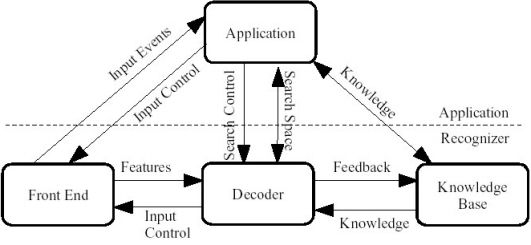
\includegraphics[width=0.8\linewidth]{sphinx_structure.png}}
\caption{Sphinx Structure \cite{understand_sphinx}.}
\label{fig:sphinx_struc}
\end{figure}

\subsubsection*{The Front End: Spectral analysis and feature extraction}
The Front End is responsible for processing the input signal so as to give the decoder understandable information. The waveform of the signal is split into utterances. Utterances are separated by silences. Then, sphinx uses basically frame-base processing, i.e. one utterance is regularly divided into frames of length 10ms before features are extracted from each frame. The feature vector is typically of length 39. The vector features used in Sphinx are extracted from spectral analysis of the frames. There are: the Mel Frequency Cepstrum Coefficients, their first and second derivatives with respect to time (Delta and Delta-Delta coefficients) and the power coefficient (or energy) with its derivatives. Figure \ref{fig:sig_proc_sphx} resumes this processing. 

\begin{figure}[h!]
\center{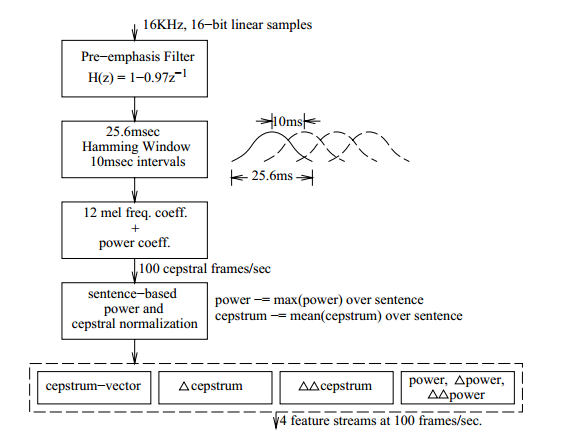
\includegraphics[width=0.8\linewidth]{signal_proc_sphinx.png}}
\caption{Signal processing in the Front End of Sphinx \cite{eff_algo}.}
\label{fig:sig_proc_sphx}
\end{figure}

\subsubsection*{The knowledge base: Different models}
The knowledge base contains three different models which will then be used by the decoder to match the given list of feature vectors to the most probable sentence. Different models are used depending on the application (language, possible vocabulary...).  

\textbf{The acoustic model}

The goal of the acoustic model is to represent the probability of a sound given a segment. In Sphinx, each phoneme is formed with five segments or states. Depending on the wideness of the vocabulary, the memory and the accuracy requirement in our application we may use either context-independent or context-dependent models. Context-dependent models aim to represent co-articulation by duplicating each phoneme model depending on its left and right contexts: triphone. Acoustic models are heavily dependent on the language and on the the way of recording. With Sphinx full acoustic models have already been trained in several languages and different recording context. It is however possible to train its own acoustic model using SphinxTrain. 

Context-independent phones and triphones in the acoustic model are represented via continuous density hidden Markov models (Figure \ref{fig:HMM}) where the transition probabilities in the model are approximated by Gaussian mixtures. In fact, Sphinx uses semi-continuous modeling with clustering. For fully continuous HMMs, each state in the HMM (i.e. each phone or triphone) needs its own separate weighted Gaussian mixture which is computationally and memory expensive. In Sphinx, the states are grouped into clusters called senones. Each senone is represented by a single Gaussian mixture codebook but inside the senone each state is represented by its own mixture weights. 

All the parameters of the HMMs are evaluated through a modified version of the Baum-Welch algorithm. 


\begin{figure}[h!]
\center{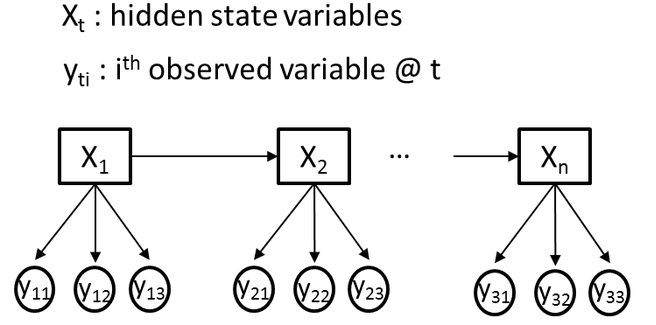
\includegraphics[width=0.5\linewidth]{HMM.png}}
\caption{Hidden Markov Model.}
\label{fig:HMM}
\end{figure}

\textbf{The lexical model}

The lexical model in sphinx consists in a phonetic dictionary. It contains a mapping from words to phones. This mapping is not very efficient because only two to three pronunciation variants are noted in it, but it is practical enough most of the time. The dictionary is not the only variant of mapper from words to phones. It could be done with some complex functions learned with a machine learning algorithm. 

\textbf{The language model}
 
The language model or grammar enables the recognizer to choose the most likely word sequence given the sounds and the previously recognized words. The language model is key in the recognition process because it makes it possible to significantly restrict the search space. By default, Sphinx uses trigrams, i.e. one computes the probability of one word occurrence given the two previous ones and forgets about earlier words.  

\subsubsection*{The decoder: Recognition itself}
The decoder performs the main part of the speech recognition. It reads features from the Front End, couples this with data from the knowledge base, and performs a search to determine the most likely sequences of words that could be represented by the series of features output by the Front End.

Sphinx recognition system has a three-pass decoder structure. The first pass consist in a forward Viterbi beam search performed on the full vocabulary. The result of this search is a single recognition hypothesis and word lattice that contains all the words recognized during the search. The second pass is a time synchronous Viterbi beam search in the backward direction. This search is restricted to the words identified in the first pass and is thus very fast. The last pass is an A* or stack search using the word segmentations and scores produced by the forward and backward Viterbi passes above. This pass outputs a list of the most likely hypothesis.

\section*{Game implementation}
We decided to play the game with 7 different colors and to display the words one by one. The recognizer to be build is then quite easy. It has a short dictionary of only five words and a grammar of only one word by a sentence. Moreover, the probability to appear for each word is the same. Thus, there is no need of building any language model in our case.

%%acoustic model -> one fitted for microphone reccrding 8khz. 

\section*{Performance analysis}
\subsection*{Theoretical Background}
When it comes to accuracy analysis of a recognizer two classical characteristics are used : The Word error rate, $WER$, and the Accuracy, $Acc$. If we call $N$ the number of words in a sentence, $D$ the number of deletions, $I$ the number of insertions and $S$ the number of substitution, those two characteristic are computed as follow: 
\begin{align*}
WER = \frac{(I + D + S)}{N},
Acc = \frac{(N-D-S)}{N}.
\end{align*}

To compute the $I$, $D$ and $S$, one 
Accuracy is actually a worse measure for most tasks, since insertions are also important in final results. But for some tasks, accuracy is a reasonable measure of the decoder performance. 

\subsection*{One word grammar}
In the game, our grammar is very basic. It consist of sentences of only one word. The possible words are the eight colors : Black, Blue, Pink, Green, White, Orange, Yellow, Red. Our first task was to analyze the accuracy of the model for the framework of our game. 

The results of our tests were very clear. In a quiet environment, we reached 100\% of accuracy. Even the word Black and Blue which have two common phonemes were not confused. Therefore, we decided to do a more advanced performance analysis.   

\subsection*{Sentence of several colors (fix number)}

\subsection*{Loop grammar}


\section*{Training the model}
Use Sphinx 3 coded in C. 

\begin{thebibliography}{40}
\bibitem{game_site} Game "say the color not what is written". \\ http://www.brainbashers.com/colour.asp

\bibitem{list_rec_soft} List of Speech recognition software. \\ http://en.wikipedia.org/wiki/List\_of\_speech\_recognition\_software

\bibitem{atk} ATK. \\ http://htk.eng.cam.ac.uk/develop/atk.shtml

\bibitem{google_speech_api} Google Web Speech API demonstration \\ https://www.google.com/intl/en/chrome/demos/speech.html

\bibitem{sphinx} CMU Sphinx. \\ http://cmusphinx.sourceforge.net/

\bibitem{understand_sphinx} Understanding the CMU sphinx Speech Recognition System (Chung Feng Liao) \\ http://soa.csie.org/static-resources/homework/pr/pr\_final\_report.pdf

\bibitem{eff_algo} Efficient algorithm for speech recognition (Mosur K. Ravishankar) \\ http://www.cs.cmu.edu/~rkm/th/th.pdf
\end{thebibliography}
\end{document}
